\documentclass[
11pt, % The default document font size, options: 10pt, 11pt, 12pt
%codirector, % Uncomment to add a codirector to the title page
]{charter} 




% El títulos de la memoria, se usa en la carátula y se puede usar el cualquier lugar del documento con el comando \ttitle
\titulo{Sistema de control y determinación de actitud (ADCS \textit{board})} 

% Nombre del posgrado, se usa en la carátula y se puede usar el cualquier lugar del documento con el comando \degreename
\posgrado{Carrera de Especialización en Sistemas Embebidos} 
%\posgrado{Carrera de Especialización en Internet de las Cosas} 
%\posgrado{Carrera de Especialización en Intelegencia Artificial}
%\posgrado{Maestría en Sistemas Embebidos} 
%\posgrado{Maestría en Internet de las cosas}

% Tu nombre, se puede usar el cualquier lugar del documento con el comando \authorname
\autor{Ing. Valdez Gastón} 
\usepackage{pdfpages}


% El nombre del director y co-director, se puede usar el cualquier lugar del documento con el comando \supname y \cosupname y 
%y \pertecosupname
%\pertesupname{Aerospace Laboratory} 
\director{Dr. Amilcar Rincón Charris}
\pertenenciaDirector{Aerospace Laboratory} 
% FIXME:NO IMPLEMENTADO EL CODIRECTOR ni su pertenencia
%\codirector{John Doe} % para que aparezca en la portada se debe descomentar la opción codirector en el documentclass
%\pertenenciaCoDirector{FIUBA}

% Nombre del cliente, quien va a aprobar los resultados del proyecto, se puede usar con el comando \clientename y \empclientename
\cliente{Dr. Amilcar Rincon Charris}
\empresaCliente{Aerospace Laboratory}
%\pertesupname{lalallal}
% Nombre y pertenencia de los jurados, se pueden usar el cualquier lugar del documento con el comando \jurunoname, \jurdosname y \jurtresname y \perteunoname, \pertedosname y \pertetresname.
\juradoUno{Nombre y Apellido (1)}
\pertenenciaJurUno{pertenencia (1)} 
\juradoDos{Nombre y Apellido (2)}
\pertenenciaJurDos{pertenencia (2)}
\juradoTres{Nombre y Apellido (3)}
\pertenenciaJurTres{pertenencia (3)}
 
\fechaINICIO{10 de octubre 2023}		%Fecha de inicio de la cursada de GdP \fechaInicioName
\fechaFINALPlan{5 de diciembre 2023} 	%Fecha de final de cursada de GdP
\fechaFINALTrabajo{30 de septiembre de 2024}	%Fecha de defensa pública del trabajo final


\begin{document}

\maketitle
\thispagestyle{empty}
\pagebreak


\thispagestyle{empty}
{\setlength{\parskip}{0pt}
\tableofcontents{}
}
\pagebreak


\section*{Registros de cambios}
\label{sec:registro}


\begin{table}[ht]
\label{tab:registro}
\centering
\begin{tabularx}{\linewidth}{@{}|c|X|c|@{}}
\hline
\rowcolor[HTML]{C0C0C0} 
Revisión & \multicolumn{1}{c|}{\cellcolor[HTML]{C0C0C0}Detalles de los cambios realizados} & Fecha      \\ \hline
0      & Creación del documento                                 &\fechaInicioName \\ \hline
1      & Se añade contexto en sección 1 \newline Se vuelve a redactar el primer ítem de la sección 5\newline
Sección 4 se redacta la última oración 
             & 11 de noviembre 2023\\ \hline
2      & Se redactan las secciones 5 a 9 & 11 de noviembre 2023 \\ \hline  
3      & Se completa hasta el punto 12 inclusive 
		 \newline Se cambia cubesat por CubeSat
		 \newline Se modifica la segunda sección
		 \newline Se cambia la cantidad de horas de algunas de las tareas               & 13 de noviembre 2023 \\ 


\hline
4      & Se completa el plan \newline Se modifica la figura \ref{fig:adcs} al idioma español  
\newline Se añaden tareas a la sección \ref{sec:wbs}
\newline Se modifica el diagrama \textit{Activity On Node}
\newline Se modifica la figura  \ref{fig:gannt} 	                                 & 15 de noviembre 2023 \\ \hline
\end{tabularx}
\end{table}

\pagebreak



\section*{Acta de constitución del proyecto}
\label{sec:acta}

\begin{flushright}
Buenos Aires, \fechaInicioName
\end{flushright}

\vspace{2cm}

Por medio de la presente se acuerda con el \authorname\hspace{1px} que su Trabajo Final de la \degreename\hspace{1px} se titulará ``\ttitle'', consiste  en el diseño electrónico de un sistema ADCS cuya funcionalidad es orientar de forma controlada un satélite denominado CubeSat y tendrá un presupuesto estimado de 600 hs de trabajo y
con fecha de inicio \fechaInicioName\hspace{1px} y fecha de presentación pública \fechaFinalName.

Se adjunta a esta acta la planificación inicial.

\vfill

% Esta parte se construye sola con la información que hayan cargado en el preámbulo del documento y no debe modificarla
\begin{table}[ht]
\centering
\begin{tabular}{ccc}
\begin{tabular}[c]{@{}c@{}}Dr. Ing. Ariel Lutenberg \\ Director posgrado FIUBA\end{tabular} & \hspace{2cm} & \begin{tabular}[c]{@{}c@{}}\clientename \\ \empclientename \end{tabular} \vspace{2.5cm} \\ 
\multicolumn{3}{c}{\begin{tabular}[c]{@{}c@{}} \supname \\ Director del Trabajo Final\end{tabular}} \vspace{2.5cm} \\
%\begin{tabular}[c]{@{}c@{}}\jurunoname \\ Jurado del Trabajo Final\end{tabular}     &  & \begin{tabular}[c]{@{}c@{}}\jurdosname\\ Jurado del Trabajo Final\end{tabular}  \vspace{2.5cm}  \\
%\multicolumn{3}{c}{\begin{tabular}[c]{@{}c@{}} \jurtresname\\ Jurado del Trabajo Final\end{tabular}} \vspace{.5cm}                                                                     
\end{tabular}
\end{table}




\section{1. Descripción técnica-conceptual del proyecto a realizar}
\label{sec:descripcion}
% agregar descripción 
%En el marco de la realización del proyecto para la aprobación de la carrera de especialización de sistemas embebidos, se ha contactado el Dr Rincon Amilcar, director del equipo PR-cunar2, perteneciente a la universidad de Puerto Rico. Esta institución se dedica a la realización de desarrollos para la industria aeroespacial. En la actualidad se encuentra en desarrollo un CubeSat que será puesto en órbita a finales del año 2024.  

El presente proyecto, se realiza para el equipo PR-cunar2, perteneciente a la Universidad de Puerto Rico. Este equipo se dedica al desarrollo de la industria aeroespacial. En este trabajo se desarrolla un módulo de hardware y software dedicado al control de la orientación de un satélite, que irá dentro de un satélite denominado CubeSat.

Un CubeSat es un satélite que posee una estructura de 10x10x10 cm y que posee un peso máximo de 1,33 kg. Los satélites CubeSat permiten que distintos investigadores y entusiastas del espacio envien satélites al espacio con un costo relativamente bajo respecto a otro tipo de soluciones. La construcción de un  CubeSat se realiza mediante módulos electrónicos ensamblados entre sí usando el bus conector denominado PC104. 

Un módulo electrónico que es parte de un CubeSat se denomina ADCS (\textit{Attitude determination control system}), este es responsable de controlar y mantener la orientación del CubeSat en el espacio. Este tipo de control  permite que los instrumentos que se encuentren dentro del satélite se orienten en direcciones específicas.  Por ejemplo puede orientar su antena hacia la tierra para que la comunicación con tierra tenga mayor fluidez. 

Los sistemas ADCS tienen dos tipos de sensores: de posicionamiento o inerciales. Los primeros se relacionan con el conocimiento de la posición absoluta, es decir, requiere un conocimiento del entorno. Los sensores inerciales no requieren este tipo de conocimiento, sino que utilizan parámetros como velocidad angular o aceleración. 

Estos sistemas no solamente deben realizar la lectura de los sensores, sino que actúan sobre el sistema para orientar el satélite en la posición deseada y mantenerla estable. Esta actuación se realiza mediante ruedas de reacción o torques magnéticos para realizar ajustes angulares cuando el satélite se encuentra orbitando la tierra.

Para generar el ajuste angular con el uso de ruedas de reacción o torques magnéticos, se debe  conocer la posición y orientación en el espacio del CubeSat. Una vez conocidos ambos parámetros, mediante un proceso denominado “algoritmo de fusión” produce la actuación sobre las ruedas de reacción o magnetorques para orientar al CubeSat en la posición deseada.

 Los sistemas ADCS se encuentran de forma comercial y  existen empresas que proveen este tipo de soluciones para los CubeSats. El presente proyecto consiste en el desarrollo de un sistema ADCS. El desarrollo propio contiene las siguientes ventajas frente a las soluciones comerciales: 
\begin{itemize}
	\item Selección de torques magnéticos, ruedas de reacción o innovar en mecanismos de orientación. 
	\item Realizar distintos algoritmos y probar la eficiencia de consumo eléctrico. 
	\item Posibilidad de generar un producto comercial. 
\end{itemize}


%El diagrama en bloques propuesto para el desarrollo del proyecto consiste en el diagrama de la figura \ref{fig:adcs}.
El diagrama en bloques del sistema ADCS se muestra en la figura \ref{fig:adcs}. El proyecto se divide en dos etapas: fase de prototipo y versión final. Una vez finalizada la fase de prototipado se realizan las pruebas de validación del sistema.  Una vez superada la etapa de validación se procede al desarrollo en su versión final y comienza la segunda fase del proyecto. 
Cabe destacar que como subproducto puede generarse una placa comercial, siendo esto último deseable pero no exigible por parte del cliente. 

\begin{figure}[htpb]
	\centering 
	\includegraphics[width=.8\textwidth]{Figuras/sistemaadcs.png}
	\caption{Diagrama en bloques del sistema a implementar.}
	\label{fig:adcs}
\end{figure}

\section{2. Identificación y análisis de los interesados}
\label{sec:interesados}
	El Dr. Amilcar Rincón Charris ocupa la posición de cliente y director. En la tabla se le ha asignado el rol de mayor importancia.


\begin{table}[ht]
	%\caption{Identificación de los interesados}
	%\label{tab:interesados}
	\begin{tabularx}{\linewidth}{@{}|l|X|X|l|@{}}
		\hline
		\rowcolor[HTML]{C0C0C0} 
		Rol           & Nombre y Apellido & Organización 	& Puesto 	\\ \hline
		Auspiciante   &  Gerardo Morell    & NASA Epscor             	& Investigador principal  \\ \hline		
%		Cliente       & \clientename      &\empclientename	& Investigador científico \\ \hline
%		Impulsor      & 	                  &              	&        	\\ \hline
		Responsable   & \authorname       & FIUBA        	& Alumno 	\\ \hline
		Colaboradores & Sebastián Medina                   &  Aerospace Laboratory        	& Asistente de laboratorio       	\\ \hline
		Orientador    & \supname	      & \pertesupname 	& Director Trabajo final \\ \hline
%		Equipo        &  -                &  -             	& -        	\\ \hline
%		Opositores    &                   &              	&        	\\ \hline
		Usuario final & Dueño de un CubeSat     &      NanoRack        	&      -   	\\ \hline
	\end{tabularx}
\end{table}


\section{3. Propósito del proyecto}

	El propósito del proyecto es generar el módulo electrónico del sistema ADCS para un CubeSat. 

\section{4. Alcance del proyecto}
\label{sec:alcance}
\begin{itemize}
	\item Desarrollo del algoritmo ADCS. 
	\item Desarrollo de software en C/C++ para el sistema embebido. 
	\item Diseño y desarrollo del protocolo de comunicación utilizando el conector PC104.
	\item Diseño y simulación del hardware asociado al microcontrolador. 
	\item Validación del producto.
	\item Generación de documentación.  
	\item Integración a un CubeSat funcional (TBD).
\end{itemize}
	
	El alcance del proyecto contempla el diseño y fabricación del PCB y	los ensayos para realizar la validación del producto se deben acordar con el cliente.  
	
\section{5. Supuestos del proyecto}
\label{sec:supuestos}
\begin{itemize}
	\item El proyecto posee financiamiento para la adquisición de productos electrónicos.   
	\item El sistema embebido posee disponibilidad en el mercado. 
	\item Se tienen las licencias correspondientes para los programas de simulación electrónica y diseño de PCB.  
	\item Se posee acceso a pc con sistema Linux/Windows. 
	\item El personal abocado al diseño mecánico realizará el trabajo en tiempo y forma.  
	\item Hay recursos económicos disponibles para enviar a fabricar la placa de circuito impreso. 
	\item Se define previamente un flujo de trabajo con el cliente. 
%	\item Se dispone del acceso al repositorio institucional del cliente 
\end{itemize}

\section{6. Requerimientos}
\label{sec:requerimientos}
	En los ítems que se enumeran a continuación se utiliza la sigla TBD (\textit{to be defined}) 
	y significa que el requerimiento aún no se terminó de acordar con el cliente. 

\begin{enumerate}
	\item Requerimientos funcionales.
		\begin{enumerate}
			\item La orientación espacial de los sensores y actuadores del CubeSat deben alinearse a los ejes principales del CubeSat.
			\item  Estimar la altitud y proporcionar control en un tiempo suficientemente corto (TBD) para que el sistema pueda controlarse exitosamente. 
			\item El control de posición se realiza en los ejes x, y, z solidarios al CubeSat.  
			\item El error máximo en la actuación del satélite será de un 10 \% respecto a la referencia elegida. 
			\item El algoritmo de control se plantea sobre CubeSat de 1 U (10x10x10 cm).
			\item La comunicación entre el ADCS y la computadora central será utilizando el protocolo SPI (opcional).  % entre uc y sensores   
			\item La comunicación con la OBC será mediante bus CAN (opcional).  
			\item Se debe utilizar un microcontrolador de bajo consumo. 
		\end{enumerate}
	\item El software debe realizarse sobre un sistema operativo de tiempo real.   
	\item El software debe gestionarse mediante un sistema de control de versiones. 
	\item Requerimientos de Test.
		\begin{enumerate}
			\item  El algoritmo de control en C/C++ debe contrastarse contra matlab u octave, scilab, etc. 
			\item  Los drivers de software deben pasar tests unitarios. 
			\item  El prototipo y su versión final debe superar el ensayo en una bobina de Helmholtz de al menos dos ejes.  
%			\item Las señales  
		\end{enumerate}
\item Requerimientos de hardware.
	\begin{enumerate}
		\item La placa de circuito impreso tendrá un tamaño máximo de 10x10 cm.
		\item El conector a utilizar es el PC104 con el estándar para CubeSats. 
		\item El PCB tendrá unívocamente identificado el eje x positivo y negativo, y positivo y negativo y z positivo y negativo. 
	\end{enumerate}

\item Requerimientos de documentación.
	\begin{enumerate}
		\item Descripción del algoritmo implementado. 
		\item Resultados del algoritmo. 
		\item Archivos de simulación y archivos de PCB. 
		\item Memoria técnica.
		\item Código fuente del sistema. 
	\end{enumerate}
\end{enumerate}



\section{7. Historias de usuarios (\textit{Product backlog})}
\label{sec:backlog}
Las historias de usuario se han escrito desde la perspectiva un ingeniero de control de misión, operador de misión espacial y científico de la misión espacial. La evaluación de las historias de usuario se evalúan en base a la complejidad de realización mediante el siguiente criterio: 
\begin{itemize}
	\item Muy bajo: 1 punto. 
	\item Bajo: 2 punto. 
	\item Medio : 3 punto. 
	\item Alto: 4 punto. 
	\item Muy alto: 5 punto. 
\end{itemize}

\begin{itemize}

	 \item Como ingeniero de control de misión, quiero que el sistema de ADCS tenga la capacidad de realizar una calibración automática de los sensores de actitud a bordo para garantizar la precisión y confiabilidad de los datos de orientación. 
		\begin{itemize}
			\item Muy alto: 5 puntos.
		\end{itemize}
	
	
	\item Como operador de una misión espacial, necesito que el sistema de ADCS tenga la capacidad de realizar ajustes dinámicos en la orientación de la nave espacial en tiempo real. .
		\begin{itemize}
			\item Muy alto: 5 puntos.
		\end{itemize}
	\item Como científico de la misión espacial, necesito que el sistema de ADCS sea capaz de proporcionar una estabilización precisa y estable de la nave espacial durante las observaciones científicas. Durante estas observaciones, es crucial evitar cualquier tipo de movimiento o vibración que pueda afectar la calidad de los datos recopilados. 
		\begin{itemize}
			\item Muy alto: 5 puntos.
		\end{itemize}
\end{itemize}


\section{8. Entregables principales del proyecto}
\label{sec:entregables}
\begin{itemize}
	\item Archivos de simulación. 
	\item Scripts de simulación. 
	\item Archivos de esquemáticos en PDF y archivo original. 
	\item Código fuente del software. 

\end{itemize}

\section{9. Desglose del trabajo en tareas}
\label{sec:wbs}
	A continuación se enumeran las tareas con su código WBS (\textit{Work Breakdown Structure}) correspondiente.  
\begin{enumerate}
	\item Inicio de planificación del proyecto
	\begin{enumerate}
		\item Elaboración del plan de proyecto (60 h). 
		\item Revisión del plan de proyecto (10 h).
		\item Presentación del plan de proyecto (10 h).
	\end{enumerate}
	\item Investigación preliminar.
		\begin{enumerate}
			\item Búsqueda bibliográfica sobre sistemas de coordenadas en sistemas ADCS (4 h). 
			\item Investigación de sistemas de coordenadas y algoritmos ADCS (40 h).
			\item Simulaciones con algoritmos ADCS y sistemas coordenados (40 h).   
			\item Selección de sensores, actuadores y microcontrolador para el desarrollo (40 h).					
		\end{enumerate}
	\item Diseño de software y hardware ADCS. 
		\begin{enumerate}
			\item Simulación de datos de sensores en C (20 h).
			\item Codificación del algoritmo ADCS en C (40 h). 
			\item Contraste de algoritmo contra simulaciones (10 h). 
			\item Diseño de arquitectura de software (25 h). 
			\item Codificación de drivers de sensores y actuadores (40 h). 
			\item Integración del software (30 hs). 
			\item Diseño y simulación electrónica (esquemático)  (30 h). 
			\item Diseño de PCB  (40 h). 
			\item Fabricación de PCB  (5 h). 
			\item Verificar la importación y trámites aduaneros para el envió del producto a Argentina (8 h). 
		\end{enumerate}
	\item Etapa de testing
		\begin{enumerate}
			\item Ensayo del bus de comunicación (16 h). 
			\item Búsqueda de lugares que tengan sala de ensayos  con bobina de Helmholtz de al menos dos ejes para medir microsatélites (20 h).
			\item  Medición de parámetros eléctricos y de software de la placa prototipado (20 h).
			\item  Informe con resultados y propuestas de mejoras (8 h).	
		\end{enumerate}
	\item Desarrollo final del producto. 
		\begin{enumerate}
			\item Realizar correcciones de software (25 h). 
			\item Realizar correcciones en el diseño del PCB (25 h).
			\item Fabricación del PCB (3 h). 
			\item Ensayo con bobina de Helmholtz (10 h). 		
			\item Medición de parámetros eléctricos y de software de la placa en su versión final (10 h). 
			\item Redacción de informe y memoria técnica (60 h).
			\item Presentación y defensa del trabajo ante el jurado (30 h). 
		\end{enumerate}

Cantidad total de horas: 679.  


\end{enumerate}





\section{10. Diagrama de Activity On Node}
\label{sec:AoN}
	En la figura \ref{fig:AoN} se muestra el diagrama  \textit{Activity on node}. Se omiten las tareas de escritura y presentación del plan de proyecto. Los códigos WBS utilizados son los utilizados en la sección \ref{sec:wbs}. Las siglas utilizadas en este diagrama son: 
	\begin{itemize}
		\item SC: sistema de coordenadas. 
		\item SW: software.
		\item HW: Hardware.
	\end{itemize}

La línea roja de la figura \ref{fig:AoN} se encuentra marcado el camino crítico del proyecto y tiene 541 horas de trabajo. 


\begin{figure}[htpb]
	\centering 
	\includegraphics[width=\linewidth]{Figuras/aoneps.eps}
	\caption{Diagrama de \textit{Activity on node.}}
	\label{fig:AoN}
\end{figure}





\section{11. Diagrama de Gantt}
\label{sec:gantt}
El diagrama de Gantt se ha realizado con 24 horas semanales de trabajo, con inicio el día 5 de diciembre del año 2023. Los códigos WBS son los presentados en la sección \ref{sec:wbs}. 


\begin{landscape}

	\begin{figure}[htpb]
		\centering 
		\includegraphics[trim=0mm 9.65cm 0mm 0mm,clip,width=\linewidth]{Figuras/ADCS_all.pdf}
		\caption{ Diagrama de Gantt.} 
		\label{fig:gannt}
	\end{figure}
	
\end{landscape}





\section{12. Presupuesto detallado del proyecto}
\label{sec:presupuesto}

La tabla de costos directos e indirectos es estimativa y puede variar según las necesidades del proyecto. La cotización se encuentra en dólares estadounidenses. La cotización al 16 de noviembre del año 2023 respecto al peso argentino (ARS) es de \$ 369,00 utilizando como referencia el Banco de la Nación. 

\begin{table}[htpb]
\centering
\begin{tabularx}{\linewidth}{@{}|X|c|r|r|@{}}
\hline
\rowcolor[HTML]{C0C0C0} 
\multicolumn{4}{|c|}{\cellcolor[HTML]{C0C0C0}COSTOS DIRECTOS} \\ \hline
\rowcolor[HTML]{C0C0C0} 
Descripción &
  \multicolumn{1}{c|}{\cellcolor[HTML]{C0C0C0}Cantidad} &
  \multicolumn{1}{c|}{\cellcolor[HTML]{C0C0C0}Valor unitario} &
  \multicolumn{1}{c|}{\cellcolor[HTML]{C0C0C0}Valor total} \\ \hline
 Acelerómetro/giróscopo BOSCH BMI270 & 
  \multicolumn{1}{c|}{1} &
  \multicolumn{1}{c|}{15 USD} &
  \multicolumn{1}{c|}{15 USD} \\ \hline
 Placa de desarrollo STM32 o simil de bajo consumo&
  \multicolumn{1}{c|}{1} &
  \multicolumn{1}{c|}{50 USD} &
  \multicolumn{1}{c|}{50 USD} \\ \hline
 Conector PC104 & 1	 
   & \multicolumn{1}{c|}{20 USD}
   & \multicolumn{1}{c|}{20 USD}
   \\ \hline
 Sensor solar & 3  
   & \multicolumn{1}{c|}{4 USD} 
   & \multicolumn{1}{c|}{12 USD} 
   \\ \hline
 Horas de ingeniería & 600  
 & \multicolumn{1}{c|}{4 USD} 
 & \multicolumn{1}{c|}{2400 USD} 
 \\ \hline

\multicolumn{3}{|c|}{SUBTOTAL} & 
\multicolumn{1}{c|}{2497 USD} \\ \hline
\rowcolor[HTML]{C0C0C0} 
\multicolumn{4}{|c|}{\cellcolor[HTML]{C0C0C0}COSTOS INDIRECTOS} \\ \hline
\rowcolor[HTML]{C0C0C0} 
Descripción &
  \multicolumn{1}{c|}{\cellcolor[HTML]{C0C0C0}Cantidad} &
  \multicolumn{1}{c|}{\cellcolor[HTML]{C0C0C0}Valor unitario} &
  \multicolumn{1}{c|}{\cellcolor[HTML]{C0C0C0}Valor total} \\ \hline
Fabricación PCB con envío & \multicolumn{1}{c|}{10} 
   & \multicolumn{1}{c|}{-} 
   & \multicolumn{1}{c|}{50 USD} 
   \\ \hline
Componentes electrónicos varios  & \multicolumn{1}{c|}{40}
   &\multicolumn{1}{c|}{-}
   &\multicolumn{1}{c|}{50 USD}
   \\ \hline
\multicolumn{3}{|c|}{SUBTOTAL} &
  \multicolumn{1}{c|}{100 USD} \\ \hline
\rowcolor[HTML]{C0C0C0}
\multicolumn{3}{|c|}{TOTAL} & 2597 USD
   \\ \hline
\end{tabularx}%
\end{table}


\section{13. Gestión de riesgos}
\label{sec:riesgos}

Riesgo 1: selección incorrecta del microcontrolador.  
\begin{itemize}
	 \item Severidad (S): 8.
	 \newline Si el microcontrolador se selecciona de forma inadecuada pueden existir problemas sobre otras partes del sistema.  
	 \item Ocurrencia (O): 4.\newline 
	 	Se  va a seleccionar un microcontrolador que este probado en ámbitos aeroespaciales y  tenga soporte del fabricante.
\end{itemize}

Riesgo 2: imposibilidad de importar el PCB poblado a Argentina.
\begin{itemize}
	\item Severidad (S): 10.
	\newline Si no fuera posible por razones normativas generar la importación del PCB poblado a Argentina se deben reorganizar las tareas con código WBS 3 y 4.
	\item Ocurrencia (O): 9.\newline 
	Ocurrió en proyectos anteriores donde el producto importado quedó retenido en la aduana, con aranceles prohibitivos para su liberación. 
\end{itemize}


Riesgo 3: diseño y simulación electrónica. 
\begin{itemize}
	\item Severidad (S): 8.
	\newline 
	Los componentes seleccionados para el diseño del PCB no los posee el fabricante. En este caso se requiere realizar cambios en el diseño del PCB consumiendo una mayor cantidad de tiempo de la pautada.  
	\item Ocurrencia (O): 5.\newline 
	En general cuando no existen ciertos componentes el fabricante te sugiere reemplazos que deben ser  evaluados en el diseño. 
\end{itemize}

Riesgo 4: inexistencia de lugares con bobina de Helmholtz.
\begin{itemize}
	\item Severidad (S): 10.
	\newline El sistema ADCS debe probarse en este tipo de dispositivos porque emula la situación del espacio exterior.   
	\item Ocurrencia (O): 4.\newline 
	Actualmente estas instalaciones se encuentran disponibles en formato comercial o servicio. Además existen diseños y esquemáticos de su fabricación y diseño en internet que se pueden utilizar de consulta. 
\end{itemize}


Riesgo 5:  mal diseño de arquitectura de software.
\begin{itemize}
	\item Severidad (S): 7.
	\newline 
	Un mal diseño de la arquitectura de software impacta en los tiempos de la tarea 2.6, extendiendo el plazo de ejecución de la tarea.  
%	Un mal diseño de la arquitecura de software hace que los plazos se extiendan dado que puede llevar una mayor cantidad de horas de integración  
	\item Ocurrencia (O): 3.
	\newline 
	El equipo de desarrollo tiene experiencia realizando el diseño de arquitectura de software e integración de las diferentes partes de sistemas complejos. 
\end{itemize}



Riesgo 6:  subestimar el tiempo de simulación y algoritmos.
\begin{itemize}
	\item Severidad (S): 9.
	\newline Una mala estimación en estos tiempos 
	genera retrasos en todas las etapas siguientes. 
%	impide que se realice el software y hardware para realizar el hardware y software 
	\item Ocurrencia (O): 5.\newline 
	Dado que el personal posee experiencia en sistemas de coordenadas la probabilidad es baja. 
\end{itemize}






\begin{table}[htpb]
\centering



\begin{tabularx}{\linewidth}{@{}|X|c|c|c|c|c|c|@{}}
\hline
\rowcolor[HTML]{C0C0C0} 
Riesgo  & S  & O & RPN & S* & O* & RPN* \\ \hline
     1. Selección incorrecta del microcontrolador. & 8  & 4 & 32  &    &    &      \\ \hline
     2. Imposibilidad de importar el PCB poblado a Argentina. & 10 & 9 & 90  &  5  & 3   & 15     \\ \hline
     3. Diseño y simulación electrónica. & 8  & 5 & 40  &  5  & 5   & 25     \\ \hline
     4. Inexistencia de lugares con bobina de Helmholtz.& 10 & 4 & 40  &  5  & 4   & 20     \\ \hline
     5. Mal diseño de arquitecutura de software. & 7.  & 3 & 21  &     &     &      \\ \hline
     6. Subestimar el tiempo de simulación y algoritmos. & 9  & 5 & 45  &  6  & 3   & 18     \\ \hline

\end{tabularx}
\end{table}

Se tomarán medidas de mitigación en los riesgos cuyos números de RPN sean mayores a 35.

Nota: los valores marcados con (*) en la tabla corresponden luego de haber aplicado la
mitigación.

Plan de mitigación de los riesgos que originalmente excedían el RPN máximo establecido:


%% PLAN DE MITIGACION DE RIESGOS 

Riesgo 2: imposibilidad de importar el PCB poblado a Argentina.
\begin{itemize}
	\item Severidad (S): 5.
	\newline Se acordará como país de destino Estados Unidos. Se realizarán las mediciones del PCB en el laboratorio del cliente. Esta acción implica la extensión de plazos de las tareas con código 3 y 4. 
	\item Ocurrencia (O): 3.\newline 
	El cliente posee instrumental y experiencia realizando PCB, mediciones, y uso de instrumental de laboratorio. 
\end{itemize}


Riesgo 3: diseño y simulación electrónica 
\begin{itemize}
	\item Severidad (S): 5. 
	\newline 
	Se deben buscar al menos tres fabricantes de PCB y verificar cual de todos presenten la mayor cantidad de componentes posibles para realizar el poblado.   
	\item Ocurrencia (O): 3.
	\newline En experiencias pasadas, el fabricante en general posee casi todos los componentes, salvo aquellos que son específicos de ciertas áreas de la electrónica (por ejemplo componentes de RF). 
\end{itemize}



Riesgo 4: inexistencia de lugares con bobina de Helmholtz
\begin{itemize}
	\item Severidad (S): 5.
	\newline  En caso de no encontrar lugares con este tipo de facilidad, se puede desarrollar o generar una orden de compra (sujeta a restricciones de presupuesto). 
	\item Ocurrencia (O): 4.\newline 
	Los sistemas ADCS son una parte crítica de los satélites, las instalaciones 
	con este tipo de dispositivos se encuentran fácilmente. 
	%se encuentran disponibles. 
%	estas dispositivo de ensayo se encuentra fácil.
\end{itemize}


Riesgo 6:  subestimar el tiempo de simulación y algoritmos. 
\begin{itemize}
	\item Severidad (S): 6.
	\newline Se utilizarán bibliotecas implementadas o precompiladas. La desventaja es el desconocimiento de esta y se requiere un esfuerzo adicional por comprender el funcionamiento. También se debe verificar la licencia de uso del software. 
	\item Ocurrencia (O): 3.\newline 
	En general los algoritmos son conocidos y la documentación de las bibliotecas para este tipo de sistemas suele tener información clara sobre el funcionamiento interno. 
\end{itemize}




\section{14. Gestión de la calidad}
\label{sec:calidad}

	Los requerimientos 1.6 y 1.7 se utiliza el mismo método de verificación y validación. 
\begin{enumerate}

	\item Requerimientos funcionales.
	\begin{enumerate}
		\setcounter{enumii}{2}
%		\item La orientación espacial de los sensores y actuadores del CubeSat deben alinearse a los ejes principales del CubeSat. %1.1 
%		\item  Estimar la altitud y proporcionar control en un tiempo suficientemente corto (TBD) para que el sistema pueda controlarse exitosamente. %1.2  
		\item El control de posición se realiza en los ejes x, y, z solidarios al CubeSat.%1.3  
			\begin{itemize}
				\item Verificación: 
				se definen diferentes posiciones para cada uno de los ejes. Luego se procede a medir la posición final de cada eje. 
				Luego se realiza la validación midiendo la posición final de cada eje y realizando la comparación contra la seleccionada inicialmente en cada uno de los ejes. 
				\item Validación: se acordará un conjunto de puntos en el espacio y se miden las posiciones respecto a las preacordadas. El dispositivo debe orientarse según la referencia dada por el cliente. 
			\end{itemize}

		
		\item El error máximo en la actuación del satélite será de un 10 \% respecto a la referencia elegida. %1.4
			\begin{itemize}
				\item Verificación: 
				 se elige una referencia para cada eje. Una vez finalizado el control, se procede a medir su posición final. 
				 Con ambos datos se calcula el error relativo y debe ser menor a un 10\%.
				\item Validación: se acuerdan con el cliente 25 referencias distintas. El dispositivo en todos los casos debe presentar un error relativo menor al 10 \%.					
			\end{itemize}

		\setcounter{enumii}{5}
%
%		\item El algoritmo de control se plantea sobre CubeSat de 1 U (10x10x10 cm).
		\item La comunicación entre el ADCS y la computadora central será utilizando el protocolo SPI (opcional).  % entre uc y sensores   
		\item La comunicación con la OBC será mediante bus CAN (opcional).  
		\begin{itemize}
			\item Verificación: se creará un dispositivo \textit{mock} (dispositivo que simula la comunicación de la OBC) que tendrá la capacidad de comunicarse con el sistema y se leer valores de respuesta. Las peticiones y respuestas se guardan en un archivo para su análisis.   
			\item Validación: se acuerda con el cliente los comandos del dispositivo y sus respuestas. Se utiliza un \textit{mock} para generar las peticiones y  guardar las respuestas. Las peticiones y respuestas se almacenan en un archivo para el cliente.  
		\end{itemize}




		\item Se debe utilizar un microcontrolador de bajo consumo. 
		\begin{itemize}
			\item Verificación: se medirá la potencia del dispositivo con el software final cargado. Se contrastan la potencia medida contra la potencia de la hoja de datos. 
			Si existieran diferencias significativas (mayor a un 20\%) se procede buscar el origen de esta diferencia.    
			\item Validación: el consumo debe ser menor a 1 W. Se mide utilizando osciloscopio y tomando muestras de la tensión  y corriente de entrada. 
		\end{itemize}
	\end{enumerate}
	\item Requerimientos de Test.
	\begin{enumerate}
		\item  El algoritmo de control en C/C++ debe contrastarse contra matlab u octave, scilab, etc. 
			\begin{itemize}
				\item Verificación:  se generan scripts en matlab, octave o scilab. Estos scripts se contrastan contra el algoritmo desarrollado en C. El algoritmo en matlab, octave o scilab tendrá los mismos estímulos del algoritmo en lenguaje C.  
				\item Validación: se entrega el reporte del  contraste contra el algoritmo en C al cliente final en un reporte para su aprobación.  
			\end{itemize}

%		\item  Los drivers de software deben pasar tests unitarios. 
		\setcounter{enumii}{2}
		\item  El prototipo y su versión final debe superar el ensayo en una bobina de Helmholtz de al menos dos ejes.  
			\begin{itemize}
				\item Verificación: se lleva el dispositivo a ensayar a un lugar donde se realicen ensayos con bobina de Helmholtz de dos o tres ejes. Durante el ensayo se realizan mediciones sobre el dispositivo. Estas medidas se validan contra los resultados teóricos. 
				\item Validación: se entregan los valores del dispositivo bajo ensayo al cliente para que se realicen las correcciones sobre aquellos parámetros que son necesarios. 
			\end{itemize}
	\end{enumerate}
	\item Requerimientos de hardware.
	\begin{enumerate}
		\item La placa de circuito impreso tendrá un tamaño máximo de 10x10 cm.
			\begin{itemize}
				\item Validación: se realiza la medición del PCB con un calibre. 
				\item Verificación: se envía el PCB al cliente para que realice la verificación del tamaño del PCB.
			\end{itemize}
		\item El conector a utilizar es el PC104 con el estándar para CubeSats. 
			\begin{itemize}
				\item Verificación: se realiza la medición sobre el conector estandarizado y se contrasta contra la norma correspondiente al conector. Además se verificará que su ubicación en el PCB sea correcta. 
				\item Validación: se envía el PCB con el conector para verificar su integración a un CubeSat.  
			\end{itemize}
		\item El PCB tendrá unívocamente identificado el eje x positivo y negativo, y positivo y negativo y z positivo y negativo. 
			\begin{itemize}
				\item Verificación: se contrasta contra los ejes del CubeSat con el PCB fabricado.   
				\item Validación: se envía el PCB fabricado al cliente para que realice la inspección de los ejes.  
			\end{itemize}



	\end{enumerate}
	
\end{enumerate}


















\section{15. Procesos de cierre}    
\label{sec:cierre}
\begin{enumerate}
	\item Análisis de seguimiento del plan original: 
	\begin{itemize}
		\item Responsable: Valdez Gastón.
		\item Se evaluará el nivel de cumplimiento de las tareas.
		\item Se realizará una comparación de fechas en conjunto con el diagrama de Gantt. 

	\end{itemize}
	\item Se dará agradecimiento a todos los interesados, en especial al equipo de trabajo, colaboradores y consultores mencionándolos en la memoria técnica.
	\item Identificación de procesos útiles e inútiles: 
	\begin{itemize}
		\item Responsable: \supname.
		\item Detectar de los procesos, cuál de ellos puede repetirse o no en futuros desarrollos.
	\end{itemize}
	\item Se realizará la presentación pública del proyecto, dando paso a la defensa del mismo ante
jurados.
	\item Se enviarán los informes al director y a los interesados dando aviso de la finalización del proyecto.
	

\end{enumerate}


\end{document}
